\documentclass[a4paper,12pt]{scrartcl}
\usepackage{exercice_sheet}

% \usepackage{fontspec}
% 
% \setmainfont[Scale=.8]{OpenDyslexic} 

%\trait
%\section*{}
%\exo{}
%\question{}
%\subquestion{}

\date{}


% Title Page
\title{Généralités sur les fonctions}

\author{\textsc{Mathématiques}}
 
\begin{document}

\maketitle

\tableofcontents

\section{Fonction, ensemble de définition}

\subsection{Notion de fonction}\label{definition}

\begin{definition}{Fonction numérique à variable réelle}
Une fonction numérique à une variable réelle est une relation qui à chaque nombre d'un ensemble de départ $D_f$ fait correspondre un nombre d'un ensemble d'arrivée. Ce nombre est noté $f(x)$.
\end{definition}


On peut rencontrer la notation suivante: $f:x \longmapsto f(x)$ qui se lit \og{} la fonction $f$ qui à $x$ associe $f(x)$\fg{}.

Ainsi, dans le cas de la fonction inverse, les deux notations sont équivalentes:
\begin{itemize}
    \item $f(x) = \frac{1}{x}$
    \item $f:x \longmapsto \frac{1}{x}$
\end{itemize}

Vocabulaire:

\begin{itemize}
    \item $f(x)$ est appelé \textbf{image} de $x$ par la fonction $f$.
    \item $x$ est appelé \textbf{antécédent} de $f(x)$ par la fonction $f$.
\end{itemize}

\exemple{Soit la fonction $f$ définie par $f(x) = \frac{1}{x+1}$}. Calculer $f(2)$, $f(0)$ et $f(1)$. 

\cadre{3} 

\subsection{Ensemble de définition}

\begin{definition}{Ensemble de définition}
C'est l'ensemble des nombres réels qui ont une et une seule image par $f$.
\end{definition}

\exemple{} soit les fonctions $f$ et $g$ définies par $f(x) = 2x +3$   et $g(x) = \sqrt{x}$ et $h(x) = \frac{1}{x}$.

\begin{itemize}
\item l'ensemble de définition $D_f$ de la fonction $f$ est: $\mathbb{R} = ]-\infty ; +\infty[$;
\item l'ensemble de définition $D_g$ de la fonction $g$ est: $\mathbb{R}^+ = [0 ; +\infty[$;
\item l'ensemble de définition $D_h$ de la fonction $h$ est: $\mathbb{R}^* = \mathbb{R} - \{ 0 \} = ]-\infty ; 0[ \cup ] 0 ; +\infty[$, trois façon différentes d'écrire \og tous les nombres réels sauf zéro \fg{}.
\end{itemize}

\exemple{Donner les ensembles de définition des fonctions suivantes: $f(x) = \frac{1}{x-1}$, $g(x) = \frac{1}{\sqrt{x}}$ et $h:x \longmapsto \frac{1}{\sqrt{x+3}}$}

\cadre{5}

Il faut noter qu'une fonction est étudiée soit sur son ensemble de définition soit sur un ensemble inclus dans celui-ci\footnote{Cela n'aurait pas de sens d'étudier une fonction là où elle n'est pas définie.}. 

\section{Représentation graphique d'une fonction}

\begin{definition}{Représentation graphique}
La représentation graphique d'une fonction $f$ est l'ensemble des points de coordonnées $(x ; f(x))$.
\end{definition}

\exemple{Représentation graphique de la fonction $f(x) = x^2$.}

Afin de pouvoir tracer le graphe, on prend plusieurs valeurs de la variable $x$, et on calcule la valeur que la fonction $f$ lui associe. Ainsi, on remplit le tableau suivant:

\begin{center}
\begin{tabular}{|c|c|c|c|c|c|c|c|}
\hline 
$x$ & -3 & -2 & -1 & 0 & 1 & 2 & 3 \\ 
\hline 
$y = f(x)$ & 9 & 4 & 1 & 0 & 1 & 4 & 9 \\ 
\hline 
\end{tabular} 
\end{center}

Il reste maintenant à les placer sur le graphe et à les relier. 

\begin{center}
\begin{tikzpicture}
\def\xmi{-3}%xmi et xma : intervalle de définition
\def\xma{3}
\def\ymi{0}
\def\yma{9}
\pgfmathsetmacro{\lrmargin}{(\xma-\xmi)/10}%de combien la grille dépasse ?
\pgfmathsetmacro{\xlborder}{\xmi-\lrmargin}
\pgfmathsetmacro{\xrborder}{\xma+\lrmargin}

\tkzInit[xmin=\xlborder,xmax=\xrborder,ymin=\ymi,ymax=\yma]
\tkzGrid[sub,color=gray, subxstep=.5,subystep=.5]
\tkzAxeXY[very thick]
\tkzGrid

\draw [domain=\xmi:\xma, very thick, color=black!60!green, samples=400] plot(\x,{(\x)^2}) node[left] {$\mathcal{C}_f$} ;
\draw (-3,9) node{$\bullet$};
\draw (-2,4) node{$\bullet$};
\draw (-1,1) node{$\bullet$};
\draw (0,0) node{$\bullet$};
\draw (1,1) node{$\bullet$};
\draw (2,4) node{$\bullet$};
\draw (3,9) node{$\bullet$};
\end{tikzpicture}
\end{center}

Rappels: 

\begin{itemize}
\item L'axe $(Ox)$ est l'axe des abscisses, l'axe $(Oy)$ est l'axe des ordonnées
\item Si les axes $(Ox)$ et $(Oy)$ sont perpendiculaires et les unités graphiques sur ces axes sont différentes on a un repère orthogonal
\item Si les axes $(Ox)$ et $(Oy)$ sont perpendiculaires et les unités graphiques sur ces axes sont identiques on a un repère orthonormé
\end{itemize}

\section{Sens de variation}

\subsection{Croissance et décroissance d'une fonction}

Soit $I$ un intervalle et $f$ une fonction définie au moins sur $I$. 

Quels que soient $a$ et $b$ deux réels de $I$ tels que $a<b$:

\begin{itemize}
\item $f$ est croissante sur $I$ si $a<b \Rightarrow f(a) \leq f(b)$
\item $f$ est strictement croissante sur $I$ si $a<b \Rightarrow f(a) < f(b)$
\item $f$ est décroissante sur $I$ si $a<b \Rightarrow f(a) \geq f(b)$
\item $f$ est strictement décroissante sur $I$ si $a<b \Rightarrow f(a) > f(b)$
\end{itemize}

\exemple{} 

Voici quelques exemples:


\begin{tabular}{|c|c|c|}
\hline 
%graphe 1
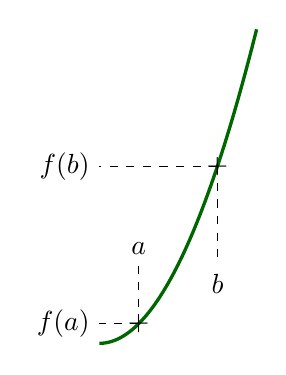
\begin{tikzpicture}
\def\xmi{0}%xmi et xma : intervalle de définition
\def\xma{2}
\def\ymi{-1}
\def\yma{3}
\pgfmathsetmacro{\lrmargin}{(\xma-\xmi)/10}%de combien la grille dépasse gauche-droite ?
\pgfmathsetmacro{\tbmargin}{(\yma-\ymi)/10}%de combien la grille dépasse haut-bas ?
\pgfmathsetmacro{\xlborder}{\xmi-\lrmargin}
\pgfmathsetmacro{\xrborder}{\xma+\lrmargin}
\pgfmathsetmacro{\ytborder}{\yma+\tbmargin}
\pgfmathsetmacro{\ybborder}{\ymi-\tbmargin}

\tkzInit[xmin=\xlborder,xmax=\xrborder,ymin=\ybborder,ymax=\ytborder]
%\tkzGrid[sub,color=gray, subxstep=.5,subystep=.5]
\tkzAxeXY[very thick]
\tkzGrid

\draw [domain=\xmi:\xma, very thick, color=black!60!green, samples=400] plot(\x,{(\x)^2 - 1});

\draw (0.5,-0.75) node{$+$};
\draw [dashed] (0.5,-0.75) -- (0.5,0)   node[above]{$a$};
\draw [dashed] (0.5,-0.75) -- (0,-0.75) node[left]{$f(a)$} ;

\draw (1.5,1.25) node{$+$};
\draw [dashed] (1.5,1.25) -- (1.5,0)   node[below]{$b$};
\draw [dashed] (1.5,1.25) -- (0,1.25) node[left]{$f(b)$} ;
\end{tikzpicture} &
%graphe 2
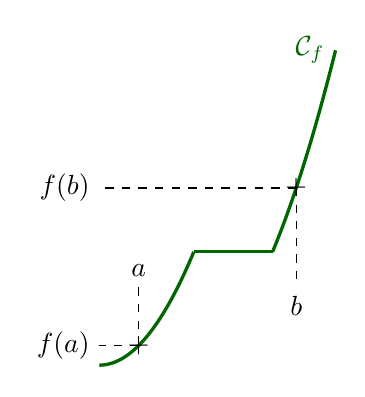
\begin{tikzpicture}
\def\xmi{0}%xmi et xma : intervalle de définition
\def\xma{3}
\def\ymi{-1}
\def\yma{3}
\pgfmathsetmacro{\lrmargin}{(\xma-\xmi)/10}%de combien la grille dépasse gauche-droite ?
\pgfmathsetmacro{\tbmargin}{(\yma-\ymi)/10}%de combien la grille dépasse haut-bas ?
\pgfmathsetmacro{\xlborder}{\xmi-\lrmargin}
\pgfmathsetmacro{\xrborder}{\xma+\lrmargin}
\pgfmathsetmacro{\ytborder}{\yma+\tbmargin}
\pgfmathsetmacro{\ybborder}{\ymi-\tbmargin}

\tkzInit[xmin=\xlborder,xmax=\xrborder,ymin=\ybborder,ymax=\ytborder]
%\tkzGrid[sub,color=gray, subxstep=.5,subystep=.5]
\tkzAxeXY[very thick]
\tkzGrid

\draw [domain=\xmi:1.2, very thick, color=black!60!green, samples=400] plot(\x,{(\x)^2 - 1});
\draw [domain=1.2:2.2, very thick, color=black!60!green, samples=400] plot(\x,{0.44});
\draw [domain=1.2:2, very thick, color=black!60!green, samples=400] plot(\x+1,{(\x)^2 - 1}) node[left] {$\mathcal{C}_f$} ;

\draw (0.5,-0.75) node{$+$};
\draw [dashed] (0.5,-0.75) -- (0.5,0)   node[above]{$a$};
\draw [dashed] (0.5,-0.75) -- (0,-0.75) node[left]{$f(a)$} ;

\draw (2.5,1.25) node{$+$};
\draw [dashed] (2.5,1.25) -- (2.5,0)   node[below]{$b$};
\draw [dashed] (2.5,1.25) -- (0,1.25) node[left]{$f(b)$} ;
\end{tikzpicture} & 
%graphe 3
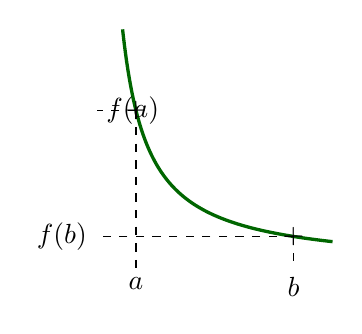
\begin{tikzpicture}
\def\xmi{.33}%xmi et xma : intervalle de définition
\def\xma{3}
\def\ymi{-1}
\def\yma{3}
\pgfmathsetmacro{\lrmargin}{(\xma-\xmi)/10}%de combien la grille dépasse gauche-droite ?
\pgfmathsetmacro{\tbmargin}{(\yma-\ymi)/10}%de combien la grille dépasse haut-bas ?
\pgfmathsetmacro{\xlborder}{\xmi-\lrmargin}
\pgfmathsetmacro{\xrborder}{\xma+\lrmargin}
\pgfmathsetmacro{\ytborder}{\yma+\tbmargin}
\pgfmathsetmacro{\ybborder}{\ymi-\tbmargin}

\tkzInit[xmin=\xlborder,xmax=\xrborder,ymin=\ybborder,ymax=\ytborder]
%\tkzGrid[sub,color=gray, subxstep=.5,subystep=.5]
\tkzAxeXY[very thick]
\tkzGrid

\draw [domain=\xmi:\xma, very thick, color=black!60!green, samples=400] plot(\x,{1/\x});

\draw (0.5,2) node{$+$};
\draw [dashed] (0.5,2) -- (0.5,0)   node[below]{$a$};
\draw [dashed] (0.5,2) -- (0,2) node[right]{$f(a)$} ;

\draw (2.5,0.4) node{$+$};
\draw [dashed] (2.5,0.4) -- (2.5,0)   node[below]{$b$};
\draw [dashed] (2.5,0.4) -- (0,0.4) node[left]{$f(b)$} ;
\end{tikzpicture} \\ 
\hline 
Strictement croissante & Croissante & Strictement décroissante \\ 
sur $[0;2]$ & sur $[0;3]$   & sur $[0;3]$  \\ 
\hline 
\end{tabular}

\subsection{Tableau de variation}

On peut résumer les variations d'une fonction dans un tableau, que l'on appelle un \emph{de variation}.

\exemple{}

Tableau de variation de la fonction $f:x \longmapsto \frac{x^3}{3} - x$ sur l'intervalle $I = [-2 ; 2]$.

\begin{center}
\simpleplot{-2.0}{2.0}{\x}{(\x)^3/3 - \x}{$\mathcal{C}_f$}{0.8}
\end{center}



On remarque que la fonction est:

\begin{itemize}
\item croissante sur $[-2 ; -1]$;
\item décroissante sur $[-1 ; 1]$;
\item croissante sur $[1 ; 2]$.
\end{itemize}

Cette information peut être résumée dans un tableau de variation:

\begin{center}
\begin{tikzpicture}
   \tkzTabInit{$x$ / 1 , $f(x)$ / 2}{$-2$, $-1$, $1$, $2$}
   \tkzTabVar{-/ $-\frac{2}{3}$, +/ $\frac{2}{3}$, -/ $-\frac{2}{3}$, +/ $\frac{2}{3}$}
\end{tikzpicture}
\end{center}

On remarque que le tableau doit si possible être complété, dans la ligne \og $f(x)$ \fg{} par les extremums de la fonction. Ici : $f(-2) = -\frac{2}{3}$, $f(-1) = \frac{2}{3}$, $f(1) = -\frac{2}{3}$ et $f(2) = \frac{2}{3}$.

\section{Opérations sur les fonctions}

\subsection{Les quatre opérations}\label{quatreOp}

On peut additionner, soustraire, multiplier ou diviser des fonctions.

\exemple{}
Soient deux fonctions $f$ et $g$ définies par $f(x) = 2x-3$ et $g(x) = 4x^2+1$.

\begin{itemize}
\item On définit la fonction somme $s = f+g$ par $s(x) = (f+g)(x) = f(x) + g(x)$.

Ainsi dans notre exemple, $s(x) = (2x-3)+(4x^2+1)$.

Soit \answer{$s(x) = 4x^2 + 2x - 2$}

\item On définit la fonction différence $d = f-g$ par $s(x) = (f-g)(x) = f(x) - g(x)$.

Ainsi dans notre exemple, $d(x) = (2x-3)-(4x^2+1)$.

Soit \answer{$d(x) = -4x^2 + 2x - 4$}

\item On définit la fonction produit $p = fg$ par $p(x) = (fg)(x) = f(x) \times g(x)$.

Ainsi dans notre exemple, $p(x) = (2x-3) \cdot (4x^2+1)$.

Soit \answer{$p(x) = (2x-3) \cdot (4x^2+1)$}

\item On définit la fonction quotient $q = \frac{f}{g}$ par $q(x) = \left( \frac{f}{g} \right)(x) = \frac{f(x)}{g(x)}$.

Ainsi dans notre exemple: \answer{$q(x) = \frac{2x-3}{4x^2+1}$}
\end{itemize}

\subsection{Composition de fonctions}

Comme vu au paragraphe \ref{definition}, une fonction est une association entre nombres de différents ensembles. Ainsi, il est tout-à-fait possible d'appliquer deux fonctions successivement:

Soient deux fonctions $f$ et $g$ et $x$ la variable. On peut appliquer $f$ et $g$ ainsi: 

$x \longmapsto f(x) \longmapsto g(f(x))$

On peut alors considérer la fonction qui à $x$ associe $g(f(x))$. Cette fonction est notée: 

\Answer{$g \circ f$}

Cela se lit \og $g$ rond $f$ \fg{}.

À noter que: 

\begin{itemize}
\item contrairement aux opérations du paragraphe \ref{quatreOp}, elle ne commute pas, c'est-à-dire que:

\begin{equation*}
g \circ f \neq f \circ g
\end{equation*}

\item dans l'exemple ci-dessus, on applique en premier la fonction $f$ et ensuite la fonction $g$. Pourtant on écrit bien $g \circ f$. En fait, la notation se comprend ainsi: $g \circ f (x) = g(f(x))$
\end{itemize}

\exemple{}
Soient les fonctions $f:x \longmapsto 3x+4$ et $g:x \longmapsto 5x-3$.

Exprimer $f \circ g (x)$ et $g \circ f (x)$ en fonction de $x$:

\cadre{8}

\section{Fonctions usuelles}

\subsection{Fonctions affines}

\subsubsection{Définition}

Ce sont les fonctions de la forme $x \longmapsto ax+b$ où $a$ et $b$ sont deux nombres réels.

\begin{itemize}
\item leur courbe représentative est toujours \textbf{une droite} non parallèle à l'axe des ordonnées;
\item $a$ est le \textbf{coefficient directeur} de la droite;
\item $b$ l'\textbf{ordonnée à l'origine} de la droite.
\end{itemize}

\begin{center}
\simpleplot{-4}{4}{\x}{0.5*(\x)+1}{$\frac{1}{2}x + 1$}{0.8}
\end{center}

\subsubsection{Cas particuliers}
\begin{itemize}
\item si $a = 0$: la fonction est constante et s'écrit sous la forme $f(x) = b$. Graphiquement, la droite est parallèle à l'axe des abscisses, ou \og horizontale. \fg{} 
\item si $b = 0$: la fonction est dite linéaire et s'écrit sous la forme $f(x) = ax$. Graphiquement, la droite passe par l'origine du repère.
\end{itemize}

\textbf{Variations:}

\begin{itemize}
\item si $a>0$, la fonction est croissante
\item si $a<0$, la fonction est décroissante
\end{itemize}

Deux droites sont \textbf{parallèles}, si et seulement si leurs \textbf{coefficients directeurs} sont \textbf{égaux}.

\subsubsection{Détermination algébrique du coefficient directeur}

Le coefficient directeur d'une droite passant par deux points $M_1(x_1;y_1)$ et $M_2(x_2;y_2)$ est donné par la relation: 

\begin{equation}
a = \frac{y_2 - y_1}{x_2 - x_1}
\end{equation}

\exemple{}
Soit une droite passant par les points $(2 ;-5) et (-1 ; 4)$. Calculer le coefficient directeur, l'ordonnée à l'origine et en déduire l'équation de la droite.

\cadre{6}

\subsubsection{Construction d'une droite à partir de son équation}

De manière générale, pour construire une droite, il faut et il suffit de deux points distincts. 

Ainsi, on choisit 2 valeurs de $x$ distinctes et on calcule les valeurs correspondantes de $y$ à partir de son équation. On place les points correspondants et on trace  la droite. 

\exemple{}
tracer la droite d'équation $y = -2x + 3$ dans le repère:

\begin{center}
\papmilli{-4}{4}{-4}{4}{1}
\end{center}

\subsubsection{Détermination algébrique des coordonnées du point d'intersection de deux droites}

Au point d'intersection, les ordonnées données par les équations des deux droites sont égales. On en déduit une équation sur $x$ que l'on résout. 

Le résultat obtenu pour $x$ permet de calculer $y$ avec l'une des deux équations.



\exemple{}
Calculer les coordonnées du point d'intersection des droites $D_1$ et $D_2$ d'équation respectives: $y = 2x -1$ et $y = -x + 5$. 

\cadre{4}

La méthode ci-dessus reste valable quel que soit le type de courbe. L'équation obtenue pourra être plus difficile à résoudre mais le principe sera toujours le même. 



\subsection{Fonctions puissance}

Ce sont les fonctions de la forme $x \longmapsto x^n$ avec $n \in \mathbb{N}$. 

La fonction carré et la fonction cube en sont des exemples:

\begin{center}
\begin{multicols}{2}
\simpleplot{-4}{4}{\x}{(\x)^2}{$x^2$}{0.8}
\simpleplot{-4}{4}{\x}{(\x)^3}{$x^3$}{0.8} 
\end{multicols}
\end{center}

\subsection{Fonction racine carrée}

La fonction racine carrée est définie sur $\mathbb{R}^+$: on \textbf{ne} peut \textbf{pas} la calculer pour des nombres négatifs.

\begin{center}
\simpleplot{0}{4}{\x}{sqrt(\x)}{$\sqrt{x}$}{0.8}
\end{center}

\subsection{Fonction inverse}

La fonction racine carrée est définie sur $\mathbb{R}^*$: on peut la calculer pour tous les nombres réels sauf 0.

\begin{center}
\simpleplot{-4}{4}{\x}{1/(\x)}{$\frac{1}{x}$}{0.8}
\end{center}

\section*{Exercices}

\exo{Déterminer l'ensemble de définition des fonctions suivantes :}
\question{}
$f(x) = \frac{2x+3}{4x+5}$

\question{}
$g(x) = \sqrt{2x+3}$

\question{}
$h(x) = \frac{4x+2}{\sqrt{2x-2}}$

\question{}
$i(x) = \frac{\sqrt{1-x}}{\sqrt{x-3}}$

\question{}
$j(x) = \sqrt{\frac{1-x}{x-3}}$

\exo{Composées de fonctions} 
On donne les fonctions $f$, $g$ et $h$ définies pour $x>0$ par $f(x) = 2x^2 + 3$, $g(x) = \frac{1}{x}$ et $h(x) = \sqrt{x}$.

Exprimer en fonction de $x$:

\begin{multicols}{3}
\question{} $f \circ g (x)$

\question{} $g \circ f (x)$

\question{} $f \circ h (x)$

\question{} $h \circ f (x)$

\question{} $g \circ h (x)$

\question{} $h \circ g (x)$
\end{multicols}

\exo{Représentations graphiques}
Soient les fonctions $f$ et $g$ définies sur $[-4 ;2]$ par $f(x) = x^2 + 2x + 1$ et $g(x) = f(x) - 2$.

\question{}
Compléter le tableau de valeurs suivant:

\begin{center}
\begin{tabular}{|c|c|c|c|c|c|c|c|}
\hline 
$x$ & -4 & -3 & -2 & -1 & 0 & 1 & 2 \\ 
\hline 
$f(x)$ & \hspace{1cm} & \hspace{1cm} & \hspace{1cm} & \hspace{1cm} & \hspace{1cm} & \hspace{1cm} & \hspace{1cm} \\ 
\hline 
$g(x)$ & \hspace{1cm} & \hspace{1cm} & \hspace{1cm} & \hspace{1cm} & \hspace{1cm} & \hspace{1cm} & \hspace{1cm} \\ 
\hline 
\end{tabular} 
\end{center}

\question{}
Représenter graphiquement les fonctions $f$ et $g$ dans un repère orthogonal. 

\begin{center}
 \papmilli{-4}{2}{-2}{9}{0.9}
\end{center}



\question{}
Par quelle transformation géométrique simple obtient-t-on la représentation graphique de la fonction $g$ à partir de celle de $f$?

\exo{Représentation graphique}
On donne  ci-dessous la représentation graphique d'une fonction $f$ définie sur l'intervalle $I = [-1 ;1]$ dans un repère.

\begin{center}
\simpleplot{-1}{1}{\x}{16*(\x)^4-8*(\x)^2}{$\mathcal{C}_f$}{2}
\end{center}

\question{}
Établir le tableau de variation de la fonction. 

\question{}
En s'aidant de la conclusion de l'exercice précédent, tracer dans le même repère la représentation graphique des fonctions $g$ et $h$ définies par: $g(x) = f(x) - 2$ et $h(x) = f(x) + 4$.

\exo{Esquisses de courbes}
Sans regarder le cours, représenter  schématiquement  de tête l'allure des représentations graphiques des fonctions suivantes:

\question{}
$f(x) = x^2$

\question{}
$g(x) = \sqrt{x}$

\question{}
$h(x) = x^3$

\question{}
$i(x) = \frac{1}{x}$

\exo{}
Écrire l'équation de la droite de coefficient directeur 3 et dont l'ordonnée à l'origine est 5.

\exo{}
Déterminer l'équation de la droite passant par les points $M(2 ;3)$ et $N(-2 ;4)$.

\exo{}
Soit la fonction $f$ définie par $f(x) = x^2 - 2$ dont la représentation graphique est la parabole $P$ donnée dans le repère ci-dessous:

\begin{center}
\simpleplot{-4}{4}{(\x)}{(\x)^2-2}{$\mathcal{C}_f$}{1}
\end{center}

\question{}
Tracer dans le même repère la droite d'équation $y = x + 3$.

\question{}
Déterminer par calcul les coordonnées des points d'intersections de la droite et de la parabole. 

\question{}
Vérifier sur le graphique et sur votre calculatrice.

\exo{}

La courbe $\mathcal{C}$ ci-dessous est la représentation graphique d'une fonction $f$ du type $f(x) = \frac{a}{x} + b$ où $a$ et $b$ sont des paramètres à déterminer. 

\begin{center}
\simpleplot{0.3}{1.8}{\x}{4/(\x)-2}{$\mathcal{C}$}{2}
\end{center}

\question{}
Sachant que la courbe $\mathcal{C}$ passe par les points $M(0,5 ; 6)$ et $N(1 ;2)$ déterminer $a$ et $b$ en résolvant un système de deux équations à deux inconnues.

\question{}
Tracer la droite $(D)$ d'équation $y = x$ dans le repère.

\question{}
Déterminer par calcul les coordonnées des points d'intersection de la droite $(D)$ et de la courbe $\mathcal{C}$.

\exo{}
On considère les fonctions $f$ et $g$ définies sur l'intervalle $[-3,8]$ par: 

$f:x \longmapsto \frac{1}{2}x+1$ et $g:x \longmapsto -\frac{1}{2}x+4$

\question{}
Représenter graphiquement les fonctions $f$ et $g$.

\question{}
Déterminer par calcul les coordonnées du point d'intersection des deux droites. Vérifier que le résultat trouvé corresponde au point d'intersection trouvé sur le graphe.

\exo{}

\question{}
Tracer dans un repère la droite $(D)$ d'équation: $y = -2x + 5$.

\question{}
Déterminer par calcul les coordonnées du point d'intersection de la droite $(D)$ avec l'axe des abscisses.

	\exo{}
	À l'aide du graphique ci-dessous déterminer l'équation des droites $D_1$ et $D_2$.

\begin{center}
       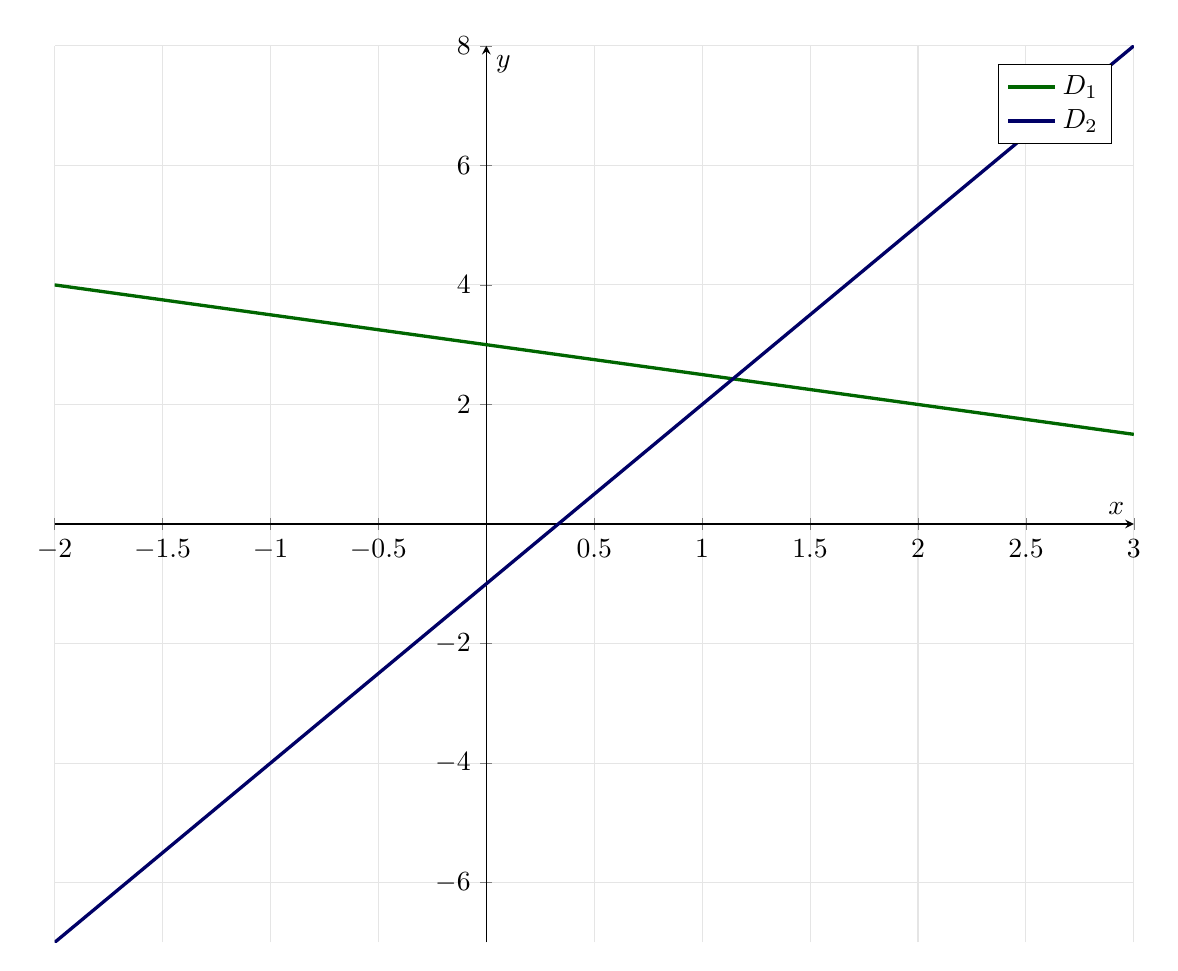
\begin{tikzpicture}[
                declare function={ 
                    X1(\x) = \x; 
                    Y1(\x) = -0.5*(\x)+3; 
                    X2(\x) = \x; 
                    Y2(\x) = 3*(\x)-1; 
            },]
            \def\xmi{-2}%xmi et xma : intervalle de définition
            \def\xma{3}

            \pgfplotsset{grid style={thin,gray!20!white}}
            \pgfplotsset{minor grid style={dotted,red}}

            \begin{axis}[
                    axis lines = center,
                    xlabel = {$x$},
                    ylabel = {$y$},    
                    grid=both,  
                    scale = 2
                ]
%First curve
                \addplot [
                    domain=\xmi:\xma, 
                    samples=400, 
                    color=black!60!green,
                    very thick,
                ]
                ({X1(\x)},{Y1(\x)});
\addlegendentry{$D_1$}
                \addplot [
                    domain=\xmi:\xma, 
                    samples=400, 
                    color=black!60!blue,
                    very thick,
                ]
                ({X2(\x)},{Y2(\x)});
\addlegendentry{$D_2$}
            \end{axis}

        \end{tikzpicture}
\end{center}

	\exo{}
	Soit la fonction $f$ définie par $f(x) = 2x^2 + 4x$ sur l'intervalle $[-3;1]$.
	
	\question{}
	Compléter le tableau suivant et représenter graphiquement la fonction. 
	
	\begin{center}
	\begin{tabular}{|c|c|c|c|c|c|}
	\hline 
	$x$ & -3 & -2 & -1 & 0 & 1 \\ 
	\hline 
	$y$ & \hspace{1cm} & \hspace{1cm} & \hspace{1cm} & \hspace{1cm} & \hspace{1cm} \\ 
	\hline 
	\end{tabular} 
	\end{center}
	
	\question{}
	Placer les points $A(-3;0)$ et $B(5,0)$ dans le repère et tracer la droite $(AB)$.
	
	\question{}
Déterminer l'équation de la droite $(AB)$.
	
	\question{}
Déterminer algébriquement les coordonnées des points d'intersection de la droite $(AB)$ et de la courbe représentative de la fonction $f$.

\exo{}
Étudier le signe des fonctions suivantes sur $]-\infty ;+\infty[$:
	
\question{}
$f(x) = 2x^2 - 7x$
	
\question{}
$g(x) = \frac{5x+3}{-2x-4}$

\exo{}
Soit la fonction $P$ telle que $P(x) = x^2 - 2x - 15$
	
\question{}
Résoudre  l'équation: $P(x) = 0$.
	
\question{}
Factoriser le polynôme $P(x)$.
	
\question{}
Étudier le signe de $P(x)$
	
\question{}
Simplifier $R(x) = \frac{x^2 - 2x - 15}{(x+2)(x-5)}$.

\exo{}
Étudier le signe des fonctions suivantes 
	
\question{}
$f_1(x) = -3x^2 - 2$
	
\question{}
$f_2(x) = \frac{4}{x^4} + 2$
	
\question{}
$f_3(x) = (1-x)^2 + 4$

\exo{}
Résoudre l'inéquation $\frac{5}{x+1} < \frac{3}{x-3}$

\exo{}
Soit la fonction polynôme définie par: $f(x) = x^3 + 4x^2 + 2x -3$.

Sa représentation graphique est donnée ci-contre.

\begin{center}
\simpleplot{-4}{1}{\x}{(\x)^3+4*(\x)^2+2*(\x)-3}{$\mathcal{C}_f$}{1.5}
\end{center}
	
\question{}
Déterminer graphiquement le nombre de solutions de l'équation $f(x) = 0$. Donner une valeur approchée de chacune d'elles.

\question{}
Déterminer des réels $a$, $b$ et $c$ pour lesquels $f(x) = (x + 3) (ax^2 + bx + c)$.

\question{}
En déduire les solutions exactes de l'équation $f(x) = 0$.

\exo{}
Résoudre les équations suivantes:

\question{}
$4x^2 - 8x - 5 = 0$

\question{}
$3x (3x + 4)  = -4$

\question{}
$(5x -1)(2x + 3) = -8$

\exo{}
Résoudre les équations suivantes (sans utiliser la méthode générale de résolution par le calcul de $\Delta$).

\question{}
$3x^2 = 15$

\question{}
$2x^2 - 5x = 0$

\question{}
$(3x - 1)(2x + 3) = 0$

\question{}
$(x+ 4)^2 - 5 = 0$

\exo{Orienté optique}
Soit l'équation :  $x^2 - 2m x + m + 2  = 0$

\question{}
Quelle valeur faut-il donner à m pour que l'équation admette 3 pour solution?

\question{}
Existe-t-il une valeur de m pour laquelle l'équation admet une seule solution?

\exo{La relation de Descartes déterminée graphiquement}

\question{}
Montrer que la relation de Descartes peut s'écrire: $\frac{f'}{p'} = -\frac{f}{p} + 1$ $f$ et $f'$ étant les distances focales objet et images, $p = HA$ et $p' = H'A'$.

\question{}
En déduire que: $p' = \frac{f' \times p}{p-f}$.

\question{}
Dans le repère ci-contre, on considère les points $M(p,0)$ et $N(f ;f')$.

\subquestion{}
Montrer que le coefficient directeur de la droite $(MN)$ est $a = \frac{f'}{f-p}$.

\subquestion{}
Montrer que l'ordonnée à l'origine de la droite $(MN)$ est $b = p' = \frac{f' \times p}{p-f}$.

\question{}
Application: on considère un dioptre sphérique de distance focale $f = -2,5$cm et $f' = 4 cm$.
Déterminer graphiquement en traçant les droites $(MN)$, la position $p'$ de l'image d'un objet dans les situations suivantes: 

\begin{itemize}
\item $p = -8$cm
\item $p = -1$cm
\item $p = 5$cm
\item $p = 2.5$cm
\item $p = \infty$
\end{itemize}

\exo{Obtenir le produit de deux nombres graphiquement}

On donne ci-contre la parabole $\mathcal{P}$ d'équation $y = x^2$.

On considère sur cette parabole deux points $M$ et $N$ d'abscisses respectives $-c$ et $d$ (où $c$ et $d$ sont deux nombres positifs).

\question{}
Montrer que le coefficient directeur de la droite $(MN)$ est $a = d - c$.

\question{}
Montrer que l'ordonnée à l'origine de la droite $(MN)$ est $b = cd$.

\question{}
Application: déterminer graphiquement le produit de $2.3 \times 1.6$ dans le repère ci-dessous: 

\begin{center}
\simpleplot{-3}{3}{\x}{(\x)^2}{$\mathcal{P}$}{2}
\end{center}

\exo{}
La courbe $\mathcal{C}$ ci-dessous est la représentation graphique d'une fonction $f$ du type $f(x) = ax^2 + bx + c$ où $a$, $b$ et $c$ sont des paramètres à déterminer. 

\begin{center}
\simpleplot{-3}{2}{\x}{2*(\x)^2+2*(\x)-4}{$\mathcal{C}$}{1.5}
\end{center}

\question{}
Sachant que la courbe $\mathcal{C}$ passe par le point $M(0 ; -4)$ déterminer $c$.

\question{}
Sachant que la courbe passe par les points $N(-1 ;-5)$  et $P(2 ; 10)$ déterminer $a$ et $b$ en résolvant un système de deux équations à deux inconnues.

\exo{}
Le but de exercice est de comparer les deux fonctions $f$ et $g$ définies sur $\mathbb{R}$ par: 

\begin{equation*}
f(x) = \frac{1}{1+x^4}
\end{equation*}

\begin{equation*}
g(x) = \frac{1}{1+x^2}
\end{equation*}

\question{}
Calculer $f(x) - g(x)$. On réduira au même dénominateur.

\question{}
En déduire l'intervalle sur lequel on a $f(x) > g(x)$.

 

\end{document}

